\documentclass[a4paper,12pt]{article}
%\documentclass[fleqn]{article}

% ---パッケージ---
\usepackage{amsmath,amssymb}    %数式用
\usepackage{tcolorbox}   %囲み枠用(tcolorboxに変更)
\usepackage{geometry}   %余白調節
\usepackage{tikz}  % ← 図を描くためのTikZパッケージ
\geometry{margin=25mm}  %余白を少し狭く
\usetikzlibrary{decorations.pathmorphing,patterns,positioning,arrows.meta} % バネ・壁の模様
\tikzset{
  block/.style = {draw, rectangle, minimum height=2em, minimum width=3em},
  sum/.style = {draw, circle, inner sep=0pt, minimum size=5mm},
  input/.style = {coordinate},
  output/.style = {coordinate}
}
\usetikzlibrary{calc}
\usepackage{pgfplots}  % ← 追加(グラフ用)
\pgfplotsset{compat=newest} % ← 推奨設定

% --- 日本語用パッケージ ---
\usepackage{luatexja}         % 日本語表示に必要
\usepackage{luatexja-fontspec} % フォント指定用

% --- フォント指定(Overleaf標準フォント)---
\setmainjfont{IPAexMincho}  % 明朝体
%\setmainjfont{IPAexGothic}  % ゴシック体にしたい場合

% --- tcolorbox の設定 ---
\tcbset{
    colframe=black,
    colback=white,         % 本文の背景(白)
    boxrule=0.8pt,
    arc=3pt,
    outer arc=3pt,
    boxsep=4pt,
    coltitle=black,
    colbacktitle=gray!20,  % タイトルの背景(グレー)
    fonttitle=\normalsize
}

\begin{document}

\noindent
\text{制御工学Ⅰ 演習① 解答}

\vspace{10mm}

\noindent
1. 以下の式に関するラプラス逆変換を求めよ.
\[
    \renewcommand{\arraystretch}{3.0} % ← 行の高さ倍率を変更(1.0が標準)
    \begin{tabular}{@{}rl@{\quad\quad}rl@{}}
    (1) & $G_1(s) = \dfrac{4}{s+5}$                 & (2) & $G_2(s) = \dfrac{s+7}{s^2+2s+5}$ \\
    (3) & $G_3(s) = \dfrac{1}{s^3+11s^2+40s+48}$    & (4) & $G_4(s) = \dfrac{1}{Ts+1} \quad [Tは定数]$ \\
    (5) & $G_5(s) = \dfrac{1}{s(s+2)(s+3)^2}$       & (6) & $G_6(s) = \dfrac{1}{(s^2+1)(s^2+4)}$ \\
    \end{tabular}
    \]\\

\begin{tcolorbox}[title={1. (1) \( G_1(s)=\frac{4}{s+5} \)}]
    \quad 両辺にラプラス逆変換を施すと,
    \vspace{-3mm}
    \begin{align*}
        &\qquad \mathcal{L}^{-1} \left[ G_1(s) \right] 
        =\mathcal{L}^{-1} \left[ \frac{4}{s+5} \right] \\
        &\Leftrightarrow x(t) = 4 e^{-5t}
    \end{align*}
\end{tcolorbox}

\begin{tcolorbox}[title={1. (2) \( G_2(s)=\frac{ s + 7 }{ s^2 + 2s + 5} \)}]
    \vspace{-3mm}
  \begin{align*}
      &\qquad G_2(s) =\frac{ s + 7 }{ s^2 + 2s + 5}  \\
      &\Leftrightarrow G_2(s) =\frac{ (s + 1) + 6 }{ ( s + 1 )^2+ 2^2} \\
      &\Leftrightarrow G_2(s) 
      = \frac{ (s + 1) }{ ( s + 1 )^2+ 2^2}
      + \frac{ 6 }{ ( s + 1 )^2+ 2^2} 
  \end{align*}
  
  \quad 両辺にラプラス逆変換を施すと,
  \vspace{-3mm}
  \begin{align*}
      &\qquad \mathcal{L}^{-1} \left[ G_2(s) \right] 
      =\mathcal{L}^{-1} \left[ \frac{ (s + 1) }{ ( s + 1 )^2+ 2^2} \right]
      +\mathcal{L}^{-1} \left[ \frac{ 6  }{ ( s + 1 )^2+ 2^2} \right] \\
      &\Leftrightarrow g_2(t) = e^{-t} cos(2t) +3 e^{-t} sin(2t)
  \end{align*}
\end{tcolorbox}

\begin{tcolorbox}[title={1. (3) \( G_3(s)=\frac{ 1 }{ s^3 + 11 s^2+ 40s + 48 } \) }]
    \vspace{-3mm}
  \begin{align*}
      &\qquad G_3(s) =\frac{ 1 }{ s^3 + 11 s^2+ 40s + 48 }  \\
      &\Leftrightarrow G_3(s) =\frac{ 1 }{ (s+3)(s+4)^2 }  \\
      &\Leftrightarrow G_3(s) 
      = \frac{1}{s+3}
      + \frac{-1}{s + 4}
      + \frac{-1}{(s + 4)^2}
      \quad [\because ヘヴィサイドの展開定理]
  \end{align*}
  
  \quad 両辺にラプラス逆変換を施すと,
  \vspace{-3mm}
  \begin{align*}
      &\qquad \mathcal{L}^{-1} \left[ G_3(s) \right] 
      =\mathcal{L}^{-1} \left[ \frac{1}{s+3} \right]
      +\mathcal{L}^{-1} \left[ \frac{-1}{s + 4} \right]
      +\mathcal{L}^{-1} \left[ \frac{-1}{(s + 4)^2} \right] \\
      &\Leftrightarrow g_3(t) = e^{-3t} - e^{-4t} - te^{-4t}
  \end{align*}
\end{tcolorbox}

\begin{tcolorbox}[title={1. (4) \( G_4(s)=\frac{1}{Ts+1} \)}]
    \begin{align*}
        &\qquad G_4(s) =\frac{1}{Ts+1}  \\
        &\Leftrightarrow G_4(s) =\frac{(\frac{1}{T})}{ s+(\frac{1}{T})} \\
    \end{align*}
    \quad 両辺にラプラス逆変換を施すと,
    \vspace{-3mm}
    \begin{align*}
        &\qquad \mathcal{L}^{-1} \left[ G_4(s) \right] 
        =\mathcal{L}^{-1} \left[ \frac{(\frac{1}{T})}{ s+(\frac{1}{T})} \right] \\
        &\Leftrightarrow g_4(t) = \frac{1}{T} e^{-\frac{t}{T}}
    \end{align*}
\end{tcolorbox}

\begin{tcolorbox}[title={1. (5) \( G_5(s)=\frac{ 1 }{ s ( s + 2 ) ( s + 3 )^2 } \) }]
    \vspace{-3mm}
  \begin{align*}
      &\qquad G_5(s) =\frac{ 1 }{ s ( s + 2 ) ( s + 3 )^2 }  \\
      &\Leftrightarrow G_5(s) 
      = \frac{\frac{1}{18}}{s}
      + \frac{(-\frac{1}{2})}{s + 2} 
      + \frac{\frac{1}{3}}{(s + 3)^2} 
      + \frac{\frac{4}{9}}{s + 3} 
  \end{align*}
  
  \quad 両辺にラプラス逆変換を施すと,
  \vspace{-3mm}
  \begin{align*}
      &\qquad \mathcal{L}^{-1} \left[ G_5(s) \right] 
      =\mathcal{L}^{-1} \left[ \frac{\frac{1}{18}}{s} \right]
      + \mathcal{L}^{-1} \left[ \frac{(-\frac{1}{2})}{s + 2} \right]
      + \mathcal{L}^{-1} \left[ \frac{\frac{1}{3}}{(s + 3)^2} \right]
      + \mathcal{L}^{-1} \left[ \frac{\frac{4}{9}}{s + 3} \right] \\
      &\Leftrightarrow g_5(t) = \frac{1}{18} - \frac{1}{2}e^{-2t} + \frac{1}{3}e^{-3t} +\frac{4}{9}e^{-3t}\\
      &\Leftrightarrow g_5(t) =\frac{1}{18} \left(1 - 9e^{-2t} + 8e^{-3t} +6te^{-3t} \right)
  \end{align*}
\end{tcolorbox}

\begin{tcolorbox}[title={1. (6) \( G_6(s)=\frac{ 1 }{ ( s^2 + 1 ) ( s^2 + 4 ) } \) }]
    \vspace{-3mm}
    \begin{align*}
      &\qquad G_6(s) =\frac{ 1 }{ ( s^2 + 1 ) ( s^2 + 4 ) } \\
      &\Leftrightarrow G_6(s) 
      = \frac{ \frac{1}{3} }{ ( s^2 + 1 ) }
      + \frac{ -\frac{1}{3} }{ ( s^2 + 4 ) }
  \end{align*}
  
  \quad 両辺にラプラス逆変換を施すと,
  \vspace{-3mm}
  \begin{align*}
      &\qquad \mathcal{L}^{-1} \left[ G_6(s) \right] 
      =\mathcal{L}^{-1} \left[ \frac{ \frac{1}{3} }{ ( s^2 + 1 ) } \right]
      +\mathcal{L}^{-1} \left[ \frac{- \frac{1}{3} }{ ( s^2 + 4 ) } \right] \\
      &\Leftrightarrow g_6(t) = \frac{1}{3}sin t -\frac{1}{6}sin 2t
  \end{align*}
  
\end{tcolorbox}

\begin{tcolorbox}[title={2. \( \ddot{y}(t) - (a+b)\dot{y}(t) + aby(t) = 0\)を解け。ただし、\(y(0)=1,\dot{y}(0)=0\)とする。
    }]
  \quad 両辺にラプラス変換を施すと,
        \vspace{-3mm}
        \begin{align*}
            &\qquad \mathcal{L}\left[ \ddot{y}(t) - ( a + b )\dot{y}(t)  + a b y(t) \right] = 0 \\
            &\Leftrightarrow \left\{ s^2 Y(s) - sy(0) - \dot{y}(0) \right\}
            - (a+b)\left\{ sY(s) - y(0) \right\}
            + abY(s) = 0  \\
            &\Leftrightarrow \left\{ s^2 - (a + b) s + ab\right\} Y(s) - s + ( a + b )= 0  \\
            &\Leftrightarrow Y(s) = \frac{s - (a + b)}{ s^2 - (a + b) s + ab }  \\
            &\Leftrightarrow Y(s) =  \frac{s - (a + b)}{ (s - a)(s - b) }  \\
            &\Leftrightarrow Y(s) =  \frac{- \frac{b}{a-b}}{ (s - a) } + \frac{ \frac{a}{a-b}}{ (s - b) }
        \end{align*}
            
        \quad 両辺にラプラス逆変換を施すと,
        \vspace{-3mm}
        \begin{align*}
        &\qquad \mathcal{L}^{-1} \left[ Y(s) \right] 
        = \mathcal{L}^{-1} \left[ \frac{- \frac{b}{a-b}}{ (s - a) } + \frac{ \frac{a}{a-b}}{ (s - b) }  \right] \\
        &\Leftrightarrow y(t) = - \frac{b}{a-b}e^{at} + \frac{a}{a-b}e^{bt}
        \end{align*}
\end{tcolorbox}

\begin{tcolorbox}[title={3. \( \ddot{x}(t) + 2\dot{x}(t) + 2x(t) = 1\)を解け。ただし、\(x(0)=0,\dot{x}(0)=1\)とする。
    }]
    \quad 両辺にラプラス変換を施すと,
    \begin{align*}
        &\qquad \mathcal{L}\left[ \frac{d^2 x(t)}{dt^2} + 2 \frac{dx(t)}{dt} + 2x(t) \right] = \mathcal{L}\{1\} \\
        &\Leftrightarrow \left\{s^2 X(s) - sx(0) - x^{(1)}(0) \right\} 
        + 2 \left\{ sX(s) - x(0) \right\} + 2X(s) 
        = \frac{1}{s} \\
        &\Leftrightarrow s^2 X(s) - 1 + 2sX(s) + 2X(s) = \frac{1}{s} \\
        &\Leftrightarrow s^2 X(s) + 2sX(s) + 2X(s) = \frac{1}{s} + 1 \\
        &\Leftrightarrow X(s) = \frac{1}{s(s^2 + 2s + 2)} + \frac{1}{s^2 + 2s + 2} \\
        &\Leftrightarrow X(s) = \frac{1}{2} \left\{ \frac{1}{s} - \frac{s+1}{(s+1)^2 + 1^2} + \frac{1}{(s+1)^2 + 1^2} \right\}
    \end{align*}
    \qquad 両辺にラプラス逆変換を施すと,
        \vspace{-3mm}
    \begin{align*}
        \mathcal{L}^{-1}\{X(s)\} = \frac{1}{2} \left\{ 1 - e^{-t}(\cos t - \sin t) \right\}
    \end{align*}
    
    
    
    \vspace{2mm}
\end{tcolorbox}

\begin{tcolorbox}[title={4. \( \dot{x}(t) + 3x(t) = \sin 2t \)を解け。ただし、\( x(0)=0 \)とする。
    }]
    \quad 両辺にラプラス変換を施すと,
    \begin{align*}
        &\qquad \mathcal{L}\left[\frac{dx(t)}{dt} + 3\mathcal{L} x(t)\right] = \mathcal{L}\{\sin 2t\} \\
        &\Leftrightarrow sX(s) - x(0) + 3X(s) = \frac{2}{s^2 + 4} \\
        &\Leftrightarrow sX(s) + 3X(s) = \frac{2}{s^2 + 4} \\
        &\Leftrightarrow X(s) = \frac{2}{(s+3)(s^2 + 4)}  \\
        &\Leftrightarrow X(s)= \frac{2}{13} \left( \frac{1}{s+3} + \frac{3}{s^2 + 4} - \frac{s}{s^2 + 4} \right) 
        \quad \left[ \because ヘヴィサイドの展開定理 \right]
    \end{align*}
        
    \quad 両辺にラプラス逆変換を施すと,
    \vspace{-3mm}
    \begin{align*}
    &\quad \mathcal{L}^{-1} \left[ X(s) \right] 
    = \mathcal{L}^{-1} \left[ \frac{2}{13} \left( \frac{1}{s+3} + \frac{3}{s^2 + 4} - \frac{s}{s^2 + 4} \right) \right] \\
    &\Leftrightarrow x(t) = \frac{1}{13} \left( 2e^{-3t} + 3\sin 2t - 2\cos 2t \right)
    \end{align*}

\vspace{2mm}
\end{tcolorbox}

\begin{tcolorbox}[title={5. あるシステムの微分方程式が\( A \ddot{y}(t) + B \dot{y}(t) + C y(t) = 1\)で表現できるとき、各パラメータを\(A=0.5,B=-0.5,C=-6,\)初期条件を\(y(0)=1,\dot{y}(0)=0\)として、\(y(t)\)
    を求めよ。 }]
    \begin{align*}
        &\qquad A \ddot{y}(t) + B \dot{y}(t) + C y(t) = 1 \\
        &\Leftrightarrow \frac{1}{2} \cdot \ddot{y}(t) - \frac{1}{2} \cdot  \dot{y}(t) - 6 y(t) = 1 \\
        &\Leftrightarrow \ddot{y}(t) - \dot{y}(t) - 12 y(t) = 2
    \end{align*}
    \quad 両辺にラプラス変換を施すと,
    \vspace{-3mm}
    \begin{align*}
        &\qquad \mathcal{L}\left[ \ddot{y}(t) - \dot{y}(t) - 12 y(t) \right] 
        = \mathcal{L} \left[ 2 \right] \\
        &\Leftrightarrow \left\{ s^2 Y(s) - sy(0) - y^{(1)}(0) \right\}
        - \left\{ sY(s) - y(0) \right\}
        - 12 Y(s) = \frac{2}{s}  \\
        &\Leftrightarrow \left\{ s^2 - s - 12 \right\} Y(s) - s + 1= \frac{2}{s}  \\
        &\Leftrightarrow Y(s) = \frac{s^2 - s + 2}{s(s^2 - s - 12)}  \\
        &\Leftrightarrow Y(s) =  \frac{s^2 - s + 2}{ s (s + 3)(s - 4) }  \\
        &\Leftrightarrow Y(s) =  \frac{- \frac{1}{6}}{ s } + \frac{  \frac{2}{3} }{ s + 3 } + \frac{  \frac{1}{2} }{ s - 4 } 
        \quad \left[\because ヘヴィサイドの展開定理 \right]
    \end{align*}
        
    \quad 両辺にラプラス逆変換を施すと,
    \vspace{-3mm}
    \begin{align*}
    &\qquad \mathcal{L}^{-1} \left[ Y(s) \right] 
    = \mathcal{L}^{-1} \left[ \frac{- \frac{1}{6}}{ s } + \frac{  \frac{2}{3} }{ s + 3 } + \frac{  \frac{1}{2} }{ s - 4 }  \right] \\
    &\Leftrightarrow y(t) = - \frac{1}{6} + \frac{2}{3}e^{-3t} + \frac{1}{2}e^{4t}
    \end{align*}
\end{tcolorbox}
6. 以下の問いに答えよ。なお、システムの入力を外力\(f(t)\)、出力を変位\(x(t)\)とする。\\
    なお、初期値はすべて\(0\)とする。\\
    \begin{center}
        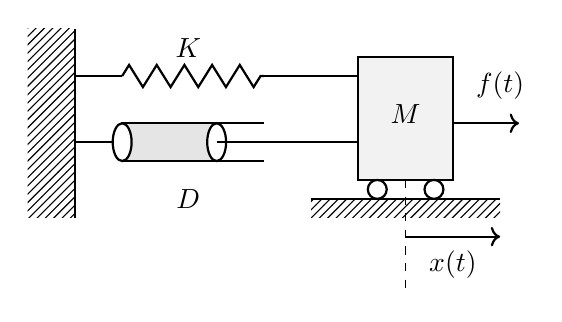
\begin{tikzpicture}[scale=1.2]
          % 固定壁
          \fill[pattern=north east lines] (-0.5,0) rectangle (0,2);
          \draw[thick] (0,0) -- (0,2);
        
          % バネ
          \draw[thick] (0,1.5) -- (0.5,1.5);
          \draw[thick, decorate, decoration={zigzag, segment length=10, amplitude=4}] (0.5,1.5) -- (2,1.5);
          \draw[thick] (2,1.5) -- (3.5,1.5);
          \node at (1.2,1.8) {$K$};
        
          % ダンパー(シリンダー形式)
          \draw[thick] (0,0.8) -- (0.5,0.8); % 棒
          \draw[thick, fill=gray!20] (0.5,0.6) rectangle (1.5,1.0); % 筒の側面
          \draw[thick] (1.5,1.0) -- (2,1.0); % 筒の上
          \draw[thick] (1.5,0.6) -- (2,0.6); % 筒の下
          \draw[thick, fill=white] (0.5,0.8) ellipse (0.1 and 0.2); % 左端面
          \draw[thick, fill=white] (1.5,0.8) ellipse (0.1 and 0.2); % 右端面
          \draw[thick] (1.5,0.8) -- (3,0.8); % ピストン棒
          \node at (1.2,0.2) {$D$};
        
          % 質量M
          \draw[thick, fill=gray!10] (3,0.4) rectangle (4,1.7);
          \node at (3.5,1.1) {$M$};
          % ローラー追加
            \draw[thick] (3.2,0.3) circle (0.1);
            \draw[thick] (3.8,0.3) circle (0.1);
    
        
          % 床
          \draw[thick] (2.5,0.2) -- (4.5,0.2);
          \fill[pattern=north east lines] (2.5,0) rectangle (4.5,0.2);
        
          % 座標
          \draw[->, thick] (3.5,-0.2) -- (4.5,-0.2);
          \node at (4,-0.5) {$x(t)$};
          \draw[dashed] (3.5,0.4) -- (3.5,-0.8);
        
          % 外力
          \draw[->, thick] (4,1) -- (4.7,1);
          \node at (4.5,1.4) {$f(t)$};
        \end{tikzpicture}
    \end{center}
    
    (1)この図によって示されるシステムの運動方程式を求めよ。\\
    
    (2)各パラメータを\(M=1,D=3,K=2,f(t)=1\)として、\(x(t)\)を求めよ。\\
    
    (3) (2)で求めた\(x(t)\)の概形を描け。なお、グラフの横軸を時間\(t\)、縦軸を変位\(x(t)\) \\
    \qquad とする。
\begin{tcolorbox}[title={6.(1)この図によって示されるシステムの運動方程式を求めよ。
    }]
    運動方程式は
    \begin{align*}
        M\ddot{x}(t) &= - Kx(t) - D \dot{x}(t) + f(t)
    \end{align*}
\end{tcolorbox}

\begin{tcolorbox}[title={6.(2)各パラメータを\(M=1,D=3,K=2,f(t)=1\)として、\(x(t)\)を求めよ。
    }]
    \begin{align*}
        &\qquad M\ddot{x}(t) = - Kx(t) - D \dot{x}(t) + f(t) \\
        &\Leftrightarrow M\ddot{x}(t) + Kx(t) + D \dot{x}(t) = f(t) \\
        &\Leftrightarrow \ddot{x}(t) + 3 \dot{x}(t) + 2x(t)= 1
    \end{align*}
    \quad 両辺にラプラス変換を施すと,
    \vspace{-3mm}
    \begin{align*}
        &\qquad \mathcal{L}\left[ \ddot{x}(t) + 3 \dot{x}(t) + 2x(t) \right] 
        = \mathcal{L} \left[ 1 \right] \\
        &\Leftrightarrow \left\{ s^2 X(s) - sx(0) - x^{(1)}(0) \right\}
        + 3\left\{ sX(s) - x(0) \right\}
        + 2 X(s) = \frac{1}{s}  \\
        &\Leftrightarrow \left\{ s^2 + 3s + 2 \right\} X(s)= \frac{1}{s}  \\
        &\Leftrightarrow X(s) = \frac{1}{s(s^2 + 3s + 2)}  \\
        &\Leftrightarrow X(s) =  \frac{1}{ s (s + 1)(s + 2) }  \\
        &\Leftrightarrow X(s) =  \frac{\frac{1}{2}}{ s } + \frac{ -1 }{ s + 1 } + \frac{  \frac{1}{2} }{ s + 2 } 
        \quad \left[\because ヘヴィサイドの展開定理 \right]
    \end{align*}
        
    \quad 両辺にラプラス逆変換を施すと,
    \vspace{-3mm}
    \begin{align*}
    &\qquad \mathcal{L}^{-1} \left[ X(s) \right] 
    = \mathcal{L}^{-1} \left[\frac{\frac{1}{2}}{ s } + \frac{ -1 }{ s + 1 } + \frac{  \frac{1}{2} }{ s + 2 }  \right] \\
    &\Leftrightarrow x(t) =\frac{1}{2}e^{-2t} - e^{-t} + \frac{1}{2}
    \end{align*}
\end{tcolorbox}

\begin{tcolorbox}[title={6.(3) (2)で求めた\(x(t)\)の概形を描け。なお、グラフの横軸を時間\(t\)、縦軸を変位\(x(t)\) 
    }]
    \begin{center}
    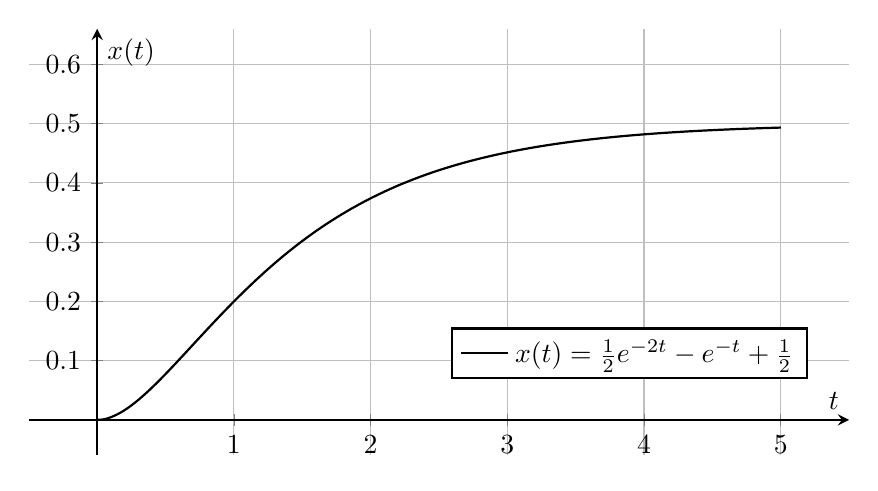
\begin{tikzpicture}
        \begin{axis}[
        axis lines=middle,
        xlabel={$t$},
        ylabel={$x(t)$},
        grid=both,
        domain=0:5,
        samples=200,
        width=12cm,
        height=7cm,
        xtick={0,1,2,3,4,5},
        ytick={0,0.1,0.2,...,0.6},
        ymin=0, ymax=0.6,
        enlargelimits=true,
        thick,
        legend style={at={(0.95,0.3)}, anchor=north east}
        ]
        \addplot[black, thick] {-exp(-x) + 0.5*exp(-2*x) + 0.5};
        \addlegendentry{$x(t) = \frac{1}{2} e^{-2t} -e^{-t}  + \frac{1}{2}$}
        \end{axis}
    \end{tikzpicture}
    \end{center}
\end{tcolorbox}

\begin{tcolorbox}[title={7.初期値を\( \dot{x}(0)=0,x(0)=1\)とするとき、微分方程式\(\ddot{x}(t)+\dot{x}(t)+x(t)=0\)を解け。 
    }]
    \quad 両辺にラプラス変換を施すと,
    \vspace{-3mm}
    \begin{align*}
        &\qquad \mathcal{L}\left[ \ddot{x}(t)+\dot{x}(t)+x(t) \right] 
        = \mathcal{L} \left[ 0 \right] \\
        &\Leftrightarrow \left\{ s^2 X(s) - sx(0) - \dot{x}(0) \right\}
        + \left\{ sX(s) - x(0) \right\}
        + X(s) = 0  \\
        &\Leftrightarrow \left\{ s^2 + s + 1 \right\} X(s) - s - 1= 0  \\
        &\Leftrightarrow \left\{ s^2 + s + 1 \right\} X(s) = s + 1 \\
        &\Leftrightarrow X(s) = \frac{s+1}{s^2 + s + 1} \\
        &\Leftrightarrow X(s) = \frac{(s+\frac{1}{2})+\frac{1}{2}}{(s+\frac{1}{2})^2+\frac{3}{4}} \\
        &\Leftrightarrow X(s) = \frac{s+\frac{1}{2}}{(s+\frac{1}{2})^2+\frac{3}{4}} 
        +\frac{1}{\sqrt{3}} \cdot \frac{\frac{\sqrt{3}}{2}}{(s+\frac{1}{2})^2+\frac{3}{4}} 
    \end{align*}
        
    \quad 両辺にラプラス逆変換を施すと,
    \vspace{-3mm}
    \begin{align*}
    &\qquad \mathcal{L}^{-1} \left[ X(s) \right] 
    = \mathcal{L}^{-1} \left[\frac{s+\frac{1}{2}}{(s+\frac{1}{2})^2+\frac{3}{4}} 
    +\frac{1}{\sqrt{3}} \cdot \frac{\frac{\sqrt{3}}{2}}{(s+\frac{1}{2})^2+\frac{3}{4}}  \right] \\
    &\Leftrightarrow x(t) =e^{-\frac{t}{2}}\left\{\cos \left(\frac{\sqrt{3}}{2}t \right)+\frac{1}{\sqrt{3}} \cdot \sin \left( \frac{\sqrt{3}}{2}t \right) \right\}
    \end{align*}
\end{tcolorbox}

\begin{tcolorbox}[title={8. \(F(s) = \frac{1}{s(s+1)^2}\)をラプラス逆変換せよ。 }]
    \vspace{-3mm}
    \begin{align*}
        &\qquad X(s) =\frac{ 1 }{ s ( s + 1 )^2 }  \\
        &\Leftrightarrow X(s) 
        = \frac{1}{s}
        + \frac{-1}{s + 1} 
        + \frac{-1}{(s + 1)^2} 
    \end{align*}
    \quad 両辺にラプラス逆変換を施すと,
    \vspace{-3mm}
    \begin{align*}
        &\qquad \mathcal{L}^{-1} \left[ X(s) \right] 
        = \mathcal{L}^{-1} \left[\frac{1}{s} \right]
        + \mathcal{L}^{-1} \left[ \frac{-1}{s + 1} \right]
        + \mathcal{L}^{-1} \left[\frac{-1}{(s + 1)^2}\right]\\
        &\Leftrightarrow x(t) = 1- e^{-t} - te^{-t}
    \end{align*}
\end{tcolorbox}
9. 下図で表される物理モデルに対する微分方程式を求め、ラプラス変換を行え。\\
    \begin{minipage}[t]{0.3\linewidth}
        (1)\\
            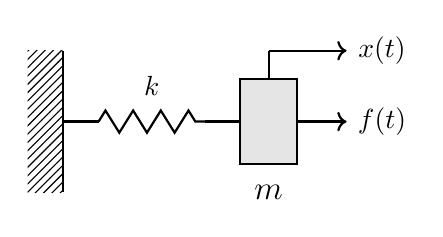
\begin{tikzpicture}[scale=0.9]
                % 固定壁
                \fill[pattern=north east lines] (-0.5,0) rectangle (0,2);
                \draw[thick] (0,0) -- (0,2);
            
                % バネ
                \draw[thick] (0,1) -- (0.5,1);
                \draw[thick, decorate, decoration={zigzag, segment length=10, amplitude=4}] (0.5,1) -- (2,1);
                \node at (1.25,1.5) {$k$};
            
                % --- 物体 ---
                \draw[thick] (2,1) -- (2.5,1); % 棒(変更なし)
                \draw[thick, fill=gray!20] (2.5,0.4) rectangle (3.3,1.6); % 筒の側面
                \node at (2.9,0) {\large $m$};
        
        
                % 入力矢印
                \draw[->, thick] (3.3,1.0) -- (4.0,1.0);
                \node at (4.5,1.0) {$f(t)$};
            
                % 出力矢印
                \draw[thick] (2.9,1.6) -- (2.9,2.0);
                \draw[->, thick] (2.9,2.0) -- (4.0,2.0);
                \node at (4.5,2.0) {$x(t)$};
            

            \end{tikzpicture}
    \end{minipage}
\hfill
    \begin{minipage}[t]{0.3\linewidth}
    (2)\\
        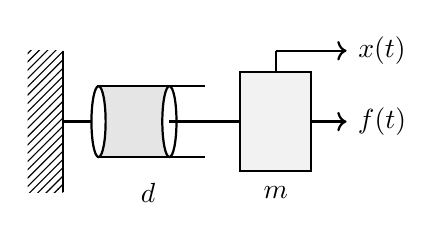
\begin{tikzpicture}[scale=0.9]
            % 固定壁
            \fill[pattern=north east lines] (-0.5,0) rectangle (0,2);
            \draw[thick] (0,0) -- (0,2);
        
            % ダンパー(シリンダー形式)
            \draw[thick] (0,1) -- (0.5,1); % 棒
            \draw[thick, fill=gray!20] (0.5,0.5) rectangle (1.5,1.5); % 筒の側面
            \draw[thick] (1.5,1.5) -- (2,1.5); % 筒の上
            \draw[thick] (1.5,0.5) -- (2,0.5); % 筒の下
            \draw[thick, fill=white] (0.5,1) ellipse (0.1 and 0.5); % 左端面
            \draw[thick, fill=white] (1.5,1) ellipse (0.1 and 0.5); % 右端面
            \draw[thick] (1.5,1) -- (2.5,1); % ピストン棒
            \node at (1.2,0) {$d$};
        
            % 質量M
            \draw[thick, fill=gray!10] (2.5,0.3) rectangle (3.5,1.7);
            \node at (3,0) {$m$};        
            % 座標
            \draw[thick] (3.0,1.7) -- (3.0,2.0);
            \draw[->, thick] (3.0,2.0) -- (4.0,2.0);
            \node at (4.5,2.0) {$x(t)$};
        
            % 外力
            \draw[->, thick] (3.5,1) -- (4.0,1);
            \node at (4.5,1) {$f(t)$};
        \end{tikzpicture}
    \end{minipage}
\hfill
\begin{minipage}[t]{0.3\linewidth}
    (3)\\
    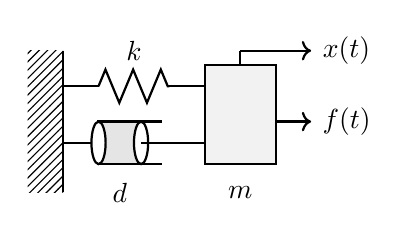
\begin{tikzpicture}[scale=0.9]
            % 固定壁
            \fill[pattern=north east lines] (-0.5,0) rectangle (0,2);
            \draw[thick] (0,0) -- (0,2);
        
            % バネ
            \draw[thick] (0,1.5) -- (0.5,1.5);
            \draw[thick, decorate, decoration={zigzag, segment length=10, amplitude=6}] (0.5,1.5) -- (1.5,1.5);
            \draw[thick] (1.5,1.5) -- (2.0,1.5);
            \node at (1.0,2.0) {$k$};
        
            % ダンパー(シリンダー形式)
            \draw[thick] (0,0.7) -- (0.5,0.7); % 棒
            \draw[thick, fill=gray!20] (0.5,0.4) rectangle (1.1,1.0); % 筒の側面
            \draw[thick] (1.1,1.0) -- (1.4,1.0); % 筒の上
            \draw[thick] (1.1,0.4) -- (1.4,0.4); % 筒の下
            \draw[thick, fill=white] (0.5,0.7) ellipse (0.1 and 0.3); % 左端面
            \draw[thick, fill=white] (1.1,0.7) ellipse (0.1 and 0.3); % 右端面
            \draw[thick] (1.1,0.7) -- (2.0,0.7); % ピストン棒
            \node at (0.8,0) {$d$};
        
            % 質量M
            \draw[thick, fill=gray!10] (2,0.4) rectangle (3,1.8);
            \node at (2.5,0) {$m$};

            % 座標
            \draw[thick] (2.5,1.8) -- (2.5,2.0);
            \draw[->, thick] (2.5,2.0) -- (3.5,2.0);
            \node at (4,2.0) {$x(t)$};
        
            % 外力
            \draw[->, thick] (3,1) -- (3.5,1);
            \node at (4.0,1.0) {$f(t)$};
    \end{tikzpicture}
\end{minipage} 
\begin{tcolorbox}[title={9.(1)
    \begin{center}
        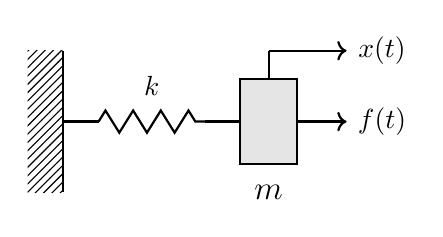
\begin{tikzpicture}[scale=0.9]
            % 固定壁
            \fill[pattern=north east lines] (-0.5,0) rectangle (0,2);
            \draw[thick] (0,0) -- (0,2);
        
            % バネ
            \draw[thick] (0,1) -- (0.5,1);
            \draw[thick, decorate, decoration={zigzag, segment length=10, amplitude=4}] (0.5,1) -- (2,1);
            \node at (1.25,1.5) {$k$};
        
            % --- 物体 ---
            \draw[thick] (2,1) -- (2.5,1); % 棒(変更なし)
            \draw[thick, fill=gray!20] (2.5,0.4) rectangle (3.3,1.6); % 筒の側面
            \node at (2.9,0) {\large $m$};
    
    
            % 入力矢印
            \draw[->, thick] (3.3,1.0) -- (4.0,1.0);
            \node at (4.5,1.0) {$f(t)$};
        
            % 出力矢印
            \draw[thick] (2.9,1.6) -- (2.9,2.0);
            \draw[->, thick] (2.9,2.0) -- (4.0,2.0);
            \node at (4.5,2.0) {$x(t)$};
        
        \end{tikzpicture}
    \end{center}}]
    運動方程式は
    \begin{align*}
        &\qquad m\ddot{x}(t) = - kx(t) + f(t)\\
        &\Leftrightarrow m\ddot{x}(t) + kx(t) = f(t)
    \end{align*}
    両辺にラプラス変換を施すと
    \begin{align*}
        &\qquad \mathcal{L} \left[ m\ddot{x}(t) + kx(t) \right] 
        = \mathcal{L} \left[f(t) \right] \\
        &\Leftrightarrow m\left\{s^2X(s)-s x(0)-\dot{x}(0)\right\}
        + k X(s)
        = F(s)\\
        &\Leftrightarrow (m s^2 + k)X(s)-mx(0)s-m\dot{x}(0)=F(s) \\
        &\Leftrightarrow (m s^2 + k)X(s) = F(s) + mx(0)s + m\dot{x}(0) \\
        &\Leftrightarrow X(s) = \frac{F(s) + mx(0)s + m\dot{x}(0)}{m s^2 + k}
    \end{align*}
\end{tcolorbox}
\begin{tcolorbox}[title={9.(2)
    \begin{center}
        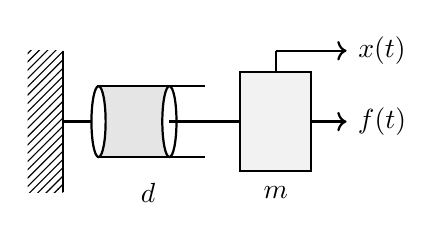
\begin{tikzpicture}[scale=0.9]
            % 固定壁
            \fill[pattern=north east lines] (-0.5,0) rectangle (0,2);
            \draw[thick] (0,0) -- (0,2);
        
            % ダンパー(シリンダー形式)
            \draw[thick] (0,1) -- (0.5,1); % 棒
            \draw[thick, fill=gray!20] (0.5,0.5) rectangle (1.5,1.5); % 筒の側面
            \draw[thick] (1.5,1.5) -- (2,1.5); % 筒の上
            \draw[thick] (1.5,0.5) -- (2,0.5); % 筒の下
            \draw[thick, fill=white] (0.5,1) ellipse (0.1 and 0.5); % 左端面
            \draw[thick, fill=white] (1.5,1) ellipse (0.1 and 0.5); % 右端面
            \draw[thick] (1.5,1) -- (2.5,1); % ピストン棒
            \node at (1.2,0) {$d$};
        
            % 質量M
            \draw[thick, fill=gray!10] (2.5,0.3) rectangle (3.5,1.7);
            \node at (3,0) {$m$};        
            % 座標
            \draw[thick] (3.0,1.7) -- (3.0,2.0);
            \draw[->, thick] (3.0,2.0) -- (4.0,2.0);
            \node at (4.5,2.0) {$x(t)$};
        
            % 外力
            \draw[->, thick] (3.5,1) -- (4.0,1);
            \node at (4.5,1) {$f(t)$};
        \end{tikzpicture}
    \end{center}}]
    運動方程式は
    \begin{align*}
        &\qquad m\ddot{x}(t) = - d \dot{x}(t) + f(t)\\
        &\Leftrightarrow m\ddot{x}(t) + d \dot{x}(t) = f(t)
    \end{align*}
    両辺にラプラス変換を施すと
    \begin{align*}
        &\qquad \mathcal{L} \left[m\ddot{x}(t) + d \dot{x}(t) \right] 
        = \mathcal{L} \left[f(t) \right] \\
        &\Leftrightarrow m\left\{s^2X(s)-s x(0)-\dot{x}(0)\right\}
        + d \left\{sX(s)-x(0)\right\}
        = F(s)\\
        &\Leftrightarrow (m s^2 + d s)X(s)-mx(0)s-m\dot{x}(0)-dx(0)=F(s) \\
        &\Leftrightarrow (m s^2 + d s)X(s) = F(s) + mx(0)s + m\dot{x}(0) + dx(0) \\
        &\Leftrightarrow X(s) = \frac{F(s) + mx(0)s + m\dot{x}(0) + dx(0)}{m s^2 + d s}
    \end{align*}
\end{tcolorbox}
\begin{tcolorbox}[title={9.(3)
    \begin{center}
    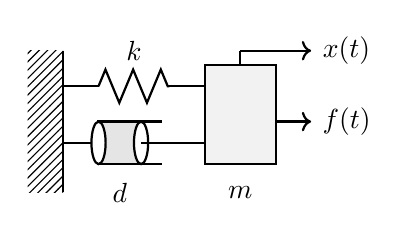
\begin{tikzpicture}[scale=0.9]
        % 固定壁
        \fill[pattern=north east lines] (-0.5,0) rectangle (0,2);
        \draw[thick] (0,0) -- (0,2);
    
        % バネ
        \draw[thick] (0,1.5) -- (0.5,1.5);
        \draw[thick, decorate, decoration={zigzag, segment length=10, amplitude=6}] (0.5,1.5) -- (1.5,1.5);
        \draw[thick] (1.5,1.5) -- (2.0,1.5);
        \node at (1.0,2.0) {$k$};
    
        % ダンパー(シリンダー形式)
        \draw[thick] (0,0.7) -- (0.5,0.7); % 棒
        \draw[thick, fill=gray!20] (0.5,0.4) rectangle (1.1,1.0); % 筒の側面
        \draw[thick] (1.1,1.0) -- (1.4,1.0); % 筒の上
        \draw[thick] (1.1,0.4) -- (1.4,0.4); % 筒の下
        \draw[thick, fill=white] (0.5,0.7) ellipse (0.1 and 0.3); % 左端面
        \draw[thick, fill=white] (1.1,0.7) ellipse (0.1 and 0.3); % 右端面
        \draw[thick] (1.1,0.7) -- (2.0,0.7); % ピストン棒
        \node at (0.8,0) {$d$};
    
        % 質量M
        \draw[thick, fill=gray!10] (2,0.4) rectangle (3,1.8);
        \node at (2.5,0) {$m$};

        % 座標
        \draw[thick] (2.5,1.8) -- (2.5,2.0);
        \draw[->, thick] (2.5,2.0) -- (3.5,2.0);
        \node at (4,2.0) {$x(t)$};
    
        % 外力
        \draw[->, thick] (3,1) -- (3.5,1);
        \node at (4.0,1.0) {$f(t)$};
    \end{tikzpicture}
    \end{center}}]
    \vspace{-3mm}
    運動方程式は
    \begin{align*}
        &\qquad m\ddot{x}(t) = -k x(t) - d \dot{x}(t) + f(t)\\
        &\Leftrightarrow m\ddot{x}(t) + d \dot{x}(t) + k x(t) = f(t)
    \end{align*}
    両辺にラプラス変換を施すと
    \vspace{-3mm}
    \begin{align*}
        &\qquad \mathcal{L} \left[ m\ddot{x}(t) + d \dot{x}(t) + k x(t) \right] 
        = \mathcal{L} \left[f(t) \right] \\
        &\Leftrightarrow m\left\{s^2X(s)-s x(0)-\dot{x}(0)\right\}
        + d \left\{sX(s)-x(0)\right\} + kX(s)
        = F(s)\\
        &\Leftrightarrow (m s^2 + d s + k)X(s)-mx(0)s-m\dot{x}(0)-dx(0)=F(s) \\
        &\Leftrightarrow (m s^2 + d s + k)X(s) = F(s) + mx(0)s + m\dot{x}(0) + dx(0) \\
        &\Leftrightarrow X(s) = \frac{F(s) + mx(0)s + m\dot{x}(0) + dx(0)}{m s^2 + d s + k}
    \end{align*}
\end{tcolorbox}

\begin{tcolorbox}[title={10.下図の物理モデルにおいて、\(f(t)\)に単位ステップ入力を印加するとき、
    \(x(t)\)を求めよ。なお、\(m=9,k=1\)とし、初期値をすべて\(0\)とする。
    \begin{center}
        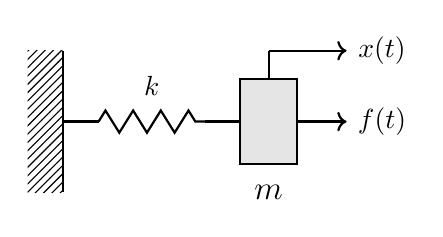
\begin{tikzpicture}[scale=0.9]
            % 固定壁
            \fill[pattern=north east lines] (-0.5,0) rectangle (0,2);
            \draw[thick] (0,0) -- (0,2);
    
            % バネ
            \draw[thick] (0,1) -- (0.5,1);
            \draw[thick, decorate, decoration={zigzag, segment length=10, amplitude=4}] (0.5,1) -- (2,1);
            \node at (1.25,1.5) {$k$};
    
            % --- 物体 ---
            \draw[thick] (2,1) -- (2.5,1); % 棒(変更なし)
            \draw[thick, fill=gray!20] (2.5,0.4) rectangle (3.3,1.6); % 筒の側面
            \node at (2.9,0) {\large $m$};
    
    
            % 入力矢印
            \draw[->, thick] (3.3,1.0) -- (4.0,1.0);
            \node at (4.5,1.0) {$f(t)$};
    
            % 出力矢印
            \draw[thick] (2.9,1.6) -- (2.9,2.0);
            \draw[->, thick] (2.9,2.0) -- (4.0,2.0);
            \node at (4.5,2.0) {$x(t)$};
    
    
        \end{tikzpicture}
    \end{center} }]
    9(1)と同様にして運動方程式は
    \vspace{-3mm}
    \begin{align*}
        &\qquad m\ddot{x}(t) = - kx(t) + f(t)
    \end{align*}
    両辺にラプラス変換を施すと
    \vspace{-3mm}
    \begin{align*}
        &\qquad \mathcal{L} \left[ m\ddot{x}(t) + kx(t) \right] 
        = \mathcal{L} \left[f(t) \right] \\
        &\Leftrightarrow m\left\{s^2X(s)-s x(0)-\dot{x}(0)\right\}
        + k X(s)
        = F(s)\\
        &\Leftrightarrow X(s) = \frac{F(s) + mx(0)s + m\dot{x}(0)}{m s^2 + k}\\
        &\Leftrightarrow X(s)= \frac{1}{s(9 s^2 + 1)} = \frac{1}{s}-\frac{9s}{9s^2 + 1}
    \end{align*}
    両辺にラプラス逆変換を施すと
    \vspace{-3mm}
    \begin{align*}
        &\qquad \mathcal{L}^{-1} \left[ X(s) \right] 
        =\mathcal{L}^{-1} \left[\frac{1}{s}-\frac{s}{s^2 + \frac{1}{9}}\right] \\
        &\Leftrightarrow x(t) = 1 - \cos \left(\frac{t}{3}\right)
    \end{align*}

\end{tcolorbox}

11.下図で表される物理モデルに対する微分方程式を求めよ。\\

\vspace{2mm}

\begin{minipage}[t]{0.45\linewidth}
    (1)\\
        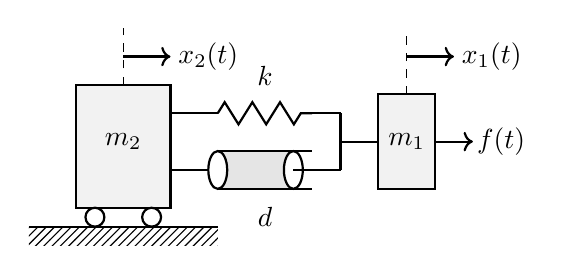
\begin{tikzpicture}[scale=1.2]
            % 質量m2
            \draw[thick, fill=gray!10] (-1,0.4) rectangle (0,1.7);
            \node at (-0.5,1.1) {$m_2$};
            % ローラー追加
            \draw[thick] (-0.8,0.3) circle (0.1);
            \draw[thick] (-0.2,0.3) circle (0.1);

            % 床
            \draw[thick] (-1.5,0.2) -- (0.5,0.2);
            \fill[pattern=north east lines] (-1.5,0) rectangle (0.5,0.2);

            % バネ
            \draw[thick] (0,1.4) -- (0.5,1.4);
            \draw[thick, decorate, decoration={zigzag, segment length=10, amplitude=4}] (0.5,1.4) -- (1.5,1.4);
            \draw[thick] (1.5,1.4) -- (1.8,1.4);
            \node at (1.0,1.8) {$k$};
        
            % ダンパー(シリンダー形式)
            \draw[thick] (0,0.8) -- (0.5,0.8); % 棒
            \draw[thick, fill=gray!20] (0.5,0.6) rectangle (1.3,1.0); % 筒の側面
            \draw[thick] (1.3,1.0) -- (1.5,1.0); % 筒の上
            \draw[thick] (1.3,0.6) -- (1.5,0.6); % 筒の下
            \draw[thick, fill=white] (0.5,0.8) ellipse (0.1 and 0.2); % 左端面
            \draw[thick, fill=white] (1.3,0.8) ellipse (0.1 and 0.2); % 右端面
            \draw[thick] (1.3,0.8) -- (1.8,0.8); % ピストン棒
            \node at (1.0,0.3) {$d$};

            %接続部分
            \draw[thick] (1.8,1.4) -- (1.8,0.8);
            \draw[thick] (1.8,1.1) -- (2.2,1.1);
        
            % 質量m1
            \draw[thick, fill=gray!10] (2.2,0.6) rectangle (2.8,1.6);
            \node at (2.5,1.1) {$m_1$};

        
            % 座標
            \draw[dashed] (-0.5,1.7) -- (-0.5,2.3);
            \draw[->, thick] (-0.5,2.0) -- (0,2.0);
            \node at (0.4,2.0) {$x_2(t)$};

            \draw[dashed] (2.5,1.6) -- (2.5,2.3);
            \draw[->, thick] (2.5,2.0) -- (3.0,2.0);
            \node at (3.4,2.0) {$x_1(t)$};

            \draw[->, thick] (2.8,1.1) -- (3.2,1.1);
            \node at (3.5,1.1) {$f(t)$};




        \end{tikzpicture}
\end{minipage}
\hfill
\begin{minipage}[t]{0.45\linewidth}
    (2)\\
        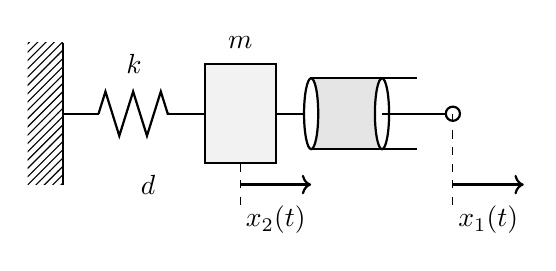
\begin{tikzpicture}[scale=0.9]
            % 固定壁
            \fill[pattern=north east lines] (-0.5,0) rectangle (0,2);
            \draw[thick] (0,0) -- (0,2);
            
            % バネ
            \draw[thick] (0,1.0) -- (0.5,1.0);
            \draw[thick, decorate, decoration={zigzag, segment length=10, amplitude=8}] (0.5,1.0) -- (1.5,1.0);
            \draw[thick] (1.5,1.0) -- (2.0,1.0);
            \node at (1.0,1.7) {$k$};
            
            % 質量M
            \draw[thick, fill=gray!10] (2.0,0.3) rectangle (3.0,1.7);
            \node at (2.5,2.0) {$m$}; 

            % ダンパー(シリンダー形式)
            \draw[thick] (3.0,1) -- (3.5,1); % 棒
            \draw[thick, fill=gray!20] (3.5,0.5) rectangle (4.5,1.5); % 筒の側面
            \draw[thick] (4.5,1.5) -- (5.0,1.5); % 筒の上
            \draw[thick] (4.5,0.5) -- (5.0,0.5); % 筒の下
            \draw[thick, fill=white] (3.5,1) ellipse (0.1 and 0.5); % 左端面
            \draw[thick, fill=white] (4.5,1) ellipse (0.1 and 0.5); % 右端面
            \draw[thick] (4.5,1) -- (5.4,1); % ピストン棒
            \node at (1.2,0) {$d$};



            \draw[thick] (5.5,1) circle (0.1);

            % 座標x_1
            \draw[dashed] (5.5,1) -- (5.5,-0.3);
            \draw[->, thick] (5.5,0) -- (6.5,0);
            \node at (6,-0.5) {$x_1(t)$};
            
            % 座標x_2
            \draw[dashed] (2.5,0.3) -- (2.5,-0.3);
            \draw[->, thick] (2.5,0) -- (3.5,0);
            \node at (3,-0.5) {$x_2(t)$};







        \end{tikzpicture}
\end{minipage}

\begin{tcolorbox}[title={11.(1)
    \begin{center}
        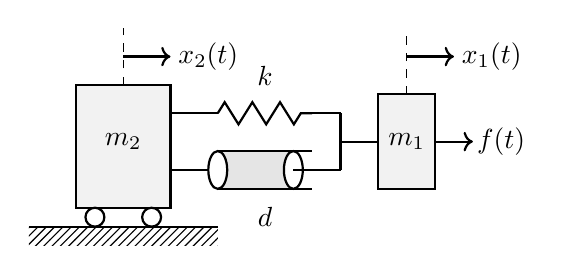
\begin{tikzpicture}[scale=1.2]
            % 質量m2
            \draw[thick, fill=gray!10] (-1,0.4) rectangle (0,1.7);
            \node at (-0.5,1.1) {$m_2$};
            % ローラー追加
            \draw[thick] (-0.8,0.3) circle (0.1);
            \draw[thick] (-0.2,0.3) circle (0.1);

            % 床
            \draw[thick] (-1.5,0.2) -- (0.5,0.2);
            \fill[pattern=north east lines] (-1.5,0) rectangle (0.5,0.2);

            % バネ
            \draw[thick] (0,1.4) -- (0.5,1.4);
            \draw[thick, decorate, decoration={zigzag, segment length=10, amplitude=4}] (0.5,1.4) -- (1.5,1.4);
            \draw[thick] (1.5,1.4) -- (1.8,1.4);
            \node at (1.0,1.8) {$k$};
        
            % ダンパー(シリンダー形式)
            \draw[thick] (0,0.8) -- (0.5,0.8); % 棒
            \draw[thick, fill=gray!20] (0.5,0.6) rectangle (1.3,1.0); % 筒の側面
            \draw[thick] (1.3,1.0) -- (1.5,1.0); % 筒の上
            \draw[thick] (1.3,0.6) -- (1.5,0.6); % 筒の下
            \draw[thick, fill=white] (0.5,0.8) ellipse (0.1 and 0.2); % 左端面
            \draw[thick, fill=white] (1.3,0.8) ellipse (0.1 and 0.2); % 右端面
            \draw[thick] (1.3,0.8) -- (1.8,0.8); % ピストン棒
            \node at (1.0,0.3) {$d$};

            %接続部分
            \draw[thick] (1.8,1.4) -- (1.8,0.8);
            \draw[thick] (1.8,1.1) -- (2.2,1.1);
        
            % 質量m1
            \draw[thick, fill=gray!10] (2.2,0.6) rectangle (2.8,1.6);
            \node at (2.5,1.1) {$m_1$};

        
            % 座標
            \draw[dashed] (-0.5,1.7) -- (-0.5,2.3);
            \draw[->, thick] (-0.5,2.0) -- (0,2.0);
            \node at (0.4,2.0) {$x_2(t)$};

            \draw[dashed] (2.5,1.6) -- (2.5,2.3);
            \draw[->, thick] (2.5,2.0) -- (3.0,2.0);
            \node at (3.4,2.0) {$x_1(t)$};

            \draw[->, thick] (2.8,1.1) -- (3.2,1.1);
            \node at (3.5,1.1) {$f(t)$};




        \end{tikzpicture}
    \end{center}}]
    運動方程式は
    \begin{align*}
        \left\{
            \begin{aligned}
        m_1 \ddot{x_1}(t) &= -k\left\{x_1(t)-x_2(t)\right\}-d\left\{\dot{x_1}(t)-\dot{x_2}(t)\right\} + f(t) \\
        m_2 \ddot{x_2}(t) &=  k\left\{x_1(t)-x_2(t)\right\}+d\left\{\dot{x_1}(t)-\dot{x_2}(t)\right\}
            \end{aligned}
        \right.
    \end{align*}
\end{tcolorbox}
\begin{tcolorbox}[title={11.(2)
    \begin{center}
        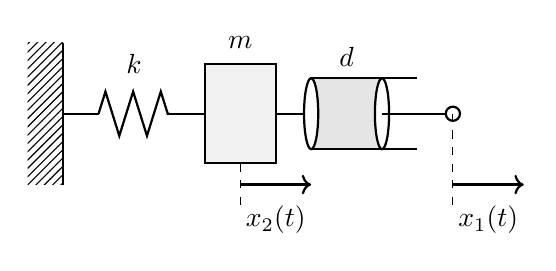
\begin{tikzpicture}[scale=0.9]
            % 固定壁
            \fill[pattern=north east lines] (-0.5,0) rectangle (0,2);
            \draw[thick] (0,0) -- (0,2);
            
            % バネ
            \draw[thick] (0,1.0) -- (0.5,1.0);
            \draw[thick, decorate, decoration={zigzag, segment length=10, amplitude=8}] (0.5,1.0) -- (1.5,1.0);
            \draw[thick] (1.5,1.0) -- (2.0,1.0);
            \node at (1.0,1.7) {$k$};
            
            % 質量M
            \draw[thick, fill=gray!10] (2.0,0.3) rectangle (3.0,1.7);
            \node at (2.5,2.0) {$m$}; 

            % ダンパー(シリンダー形式)
            \draw[thick] (3.0,1) -- (3.5,1); % 棒
            \draw[thick, fill=gray!20] (3.5,0.5) rectangle (4.5,1.5); % 筒の側面
            \draw[thick] (4.5,1.5) -- (5.0,1.5); % 筒の上
            \draw[thick] (4.5,0.5) -- (5.0,0.5); % 筒の下
            \draw[thick, fill=white] (3.5,1) ellipse (0.1 and 0.5); % 左端面
            \draw[thick, fill=white] (4.5,1) ellipse (0.1 and 0.5); % 右端面
            \draw[thick] (4.5,1) -- (5.4,1); % ピストン棒
            \node at (4.0,1.8) {$d$};

            \draw[thick] (5.5,1) circle (0.1);

            % 座標x_1
            \draw[dashed] (5.5,1) -- (5.5,-0.3);
            \draw[->, thick] (5.5,0) -- (6.5,0);
            \node at (6,-0.5) {$x_1(t)$};
            
            % 座標x_2
            \draw[dashed] (2.5,0.3) -- (2.5,-0.3);
            \draw[->, thick] (2.5,0) -- (3.5,0);
            \node at (3,-0.5) {$x_2(t)$};
        \end{tikzpicture}
    \end{center}}]
    運動方程式は
    \begin{align*}
        \left\{
            \begin{aligned}
        M \ddot{x_1}(t) &= - d \left\{\dot{x_1}(t)-\dot{x_2}(t)\right\} \\
        m \ddot{x_2}(t) &= - k x_2(t) + d \left\{\dot{x_1}(t)-\dot{x_2}(t)\right\}
            \end{aligned}
        \right.
    \end{align*}
\end{tcolorbox}
\end{document}